% UPC 2026 Problem B paper. Compile with pdfLaTeX (twice for cross-references).
% Team 155. All numbers trace to student_b/runs/*.json in the project repository.
\documentclass[11pt,a4paper]{article}

\usepackage{iftex}
\ifPDFTeX
  \usepackage[T1]{fontenc}
  \usepackage[utf8]{inputenc}
  \usepackage{lmodern}
\else
  % XeLaTeX supports Chinese text in an AI report, if needed.
  \usepackage{fontspec}
  \usepackage{xeCJK}
  \setmainfont{Latin Modern Roman}
\fi
\usepackage[margin=1in,headheight=15pt,headsep=20pt]{geometry}
\usepackage{amsmath,amssymb}
\usepackage{graphicx}
\usepackage{booktabs}
\usepackage{array}
\usepackage{float}
\usepackage{fvextra}
\usepackage{fancyhdr}
\usepackage{microtype}
\usepackage{url}
\usepackage{hyperref}
\hypersetup{hidelinks,pdfauthor={},pdftitle={},pdfsubject={},pdfkeywords={}}
\urlstyle{same}
\setlength{\parindent}{0pt}
\setlength{\parskip}{0.55em}
\setcounter{tocdepth}{2}

% ========== Fill these three fields first ==========
\newcommand{\teamnumber}{155}
\newcommand{\problemletter}{B}
\newcommand{\papertitle}{Two Points to the Goal: A Noise-Conditioned Mixture Density Network for Probabilistic Penalty Kick Prediction}
\newcommand{\todo}[1]{\textbf{[TODO: #1]}}

% Team number at the top of every page, including the first page.
\pagestyle{fancy}
\fancyhf{}
\fancyhead[L]{Team \teamnumber}
\fancyfoot[C]{\thepage}
\renewcommand{\headrulewidth}{0.4pt}
\renewcommand{\footrulewidth}{0pt}
\fancypagestyle{cover}{%
  \fancyhf{}%
  \fancyhead[L]{Team \teamnumber}%
  \renewcommand{\headrulewidth}{0pt}%
}

\begin{document}

% FIRST PAGE: only team number, problem letter, title, and summary.
% Keep the summary at or below 300 English words. Check that it fits on page 1.
\thispagestyle{cover}
\begin{center}
  \vspace*{1.0cm}
  {\large Problem \problemletter\par}
  \vspace{1.2cm}
  {\LARGE\bfseries \papertitle\par}
  \vspace{1.2cm}
  {\large\bfseries Summary\par}
\end{center}
\vspace{0.2cm}

Can the destination of a penalty kick be inferred from its first two tenths of a second? We model the ball as a point mass under gravity, quadratic drag and a transverse Magnus force, with aerodynamic coefficients taken from wind-tunnel and trajectory studies. The launch velocity, spin vector and drag coefficient are unknown; the initial position is exact, while the positions at $0.05\,\mathrm{s}$ and $0.10\,\mathrm{s}$ are observed with $2$--$15\,\mathrm{mm}$ noise. For the stated case, constant-acceleration extrapolation reaches the goal plane at $T=0.405\,\mathrm{s}$ and $(Y,Z)=(2.495,1.920)\,\mathrm{m}$.

We solve the inverse problem with two complementary estimators. A physics-constrained Bayesian sampler returns a posterior over launch conditions, and a noise-conditioned mixture density network (MDN) maps the six observed coordinates plus the noise level to a three-component, full-covariance Gaussian mixture of the crossing point. The MDN is trained on 50{,}000 simulated trajectories and evaluated on 4{,}187 held-out airborne crossings.

At $\sigma=5\,\mathrm{mm}$ the posterior mode is $(2.650,2.052)\,\mathrm{m}$, with 50\% and 95\% joint regions of $0.219$ and $0.809\,\mathrm{m^2}$; the probability that the ball centre crosses inside the goal rectangle is $0.963$. The MDN gives $(2.773,1.924)\,\mathrm{m}$ and $0.974$. On held-out trajectories the median endpoint error is $0.163$, $0.322$ and $0.556\,\mathrm{m}$ at $\sigma=2$, $5$ and $15\,\mathrm{mm}$, $14$--$54\%$ below the baseline, while 95\% coverage is $96$--$98\%$ and 50\% coverage ($47$--$59\%$) reveals residual miscalibration. Two tracked free-kick arcs confirm the drag correction (forecast RMSE $0.70\to0.49\,\mathrm{m}$ and $2.18\to1.55\,\mathrm{m}$). All results are conditioned on airborne arrival and remain simulation-calibrated rather than validated on penalty data.

\clearpage
\tableofcontents
\clearpage

\section{Introduction}
\subsection{Problem Restatement}

A penalty kick starts $11\,\mathrm{m}$ from a goal that is $7.32\,\mathrm{m}$ wide and $2.44\,\mathrm{m}$ high \cite{ifab}. Taking the penalty spot as the origin and the goal line as the plane $x=11\,\mathrm{m}$, the ball centre begins at $\mathbf{r}(0)=(0,0,0.11)\,\mathrm{m}$, and two further positions are observed: $\mathbf{r}(0.05)$ and $\mathbf{r}(0.10)$. The task is to predict the first crossing of the goal plane: the most likely point $(Y,Z)$, joint $50\%$ and $95\%$ prediction regions, and the probability that the ball passes inside the goal. The final crossing is a label for validation only; it may not be used as an input.

Two properties make this inverse problem difficult. First, the trajectory is driven by forces that are not observed. The launch speed is roughly $30\,\mathrm{m\,s^{-1}}$ \cite{bray2003}, the Reynolds number is of order $10^5$, and the drag coefficient of a football changes by a factor of almost three across the drag crisis \cite{asai2007}. Spin generates a Magnus force whose direction depends on the spin axis, which a tracking system does not measure. Second, the observations are only marginally informative. With the start fixed and two positions observed independently with standard deviation $\sigma$, the second difference that estimates acceleration carries noise $\sqrt{5}\,\sigma/\Delta t^2$ (Appendix~\ref{app:noise}). For $\sigma=5\,\mathrm{mm}$ and $\Delta t=0.05\,\mathrm{s}$ this is $4.47\,\mathrm{m\,s^{-2}}$, comparable to the aerodynamic accelerations themselves. A predictor that ignores this amplification will be overconfident.

\subsection{Background and Approach}

The aerodynamics of a football are well studied. Wind-tunnel work gives a subcritical drag coefficient near $0.43$, a supercritical value near $0.15$, and a critical Reynolds number of $2.2$--$3.0\times10^5$ \cite{asai2007,asai2013}; trajectory analyses of free kicks report effective drag coefficients of $0.25$--$0.30$ \cite{bray2003}, and lift coefficients of $0.2$--$0.3$ at moderate spin parameters \cite{goff2010}. More recent work recovers drag and lift curves directly from tracked trajectories \cite{goff2017}. These ranges, rather than a single calibrated value, define our prior. Public tracking datasets make real ball trajectories available: the ISSIA-3D annotations distributed with SoccerNet-v3D provide calibrated, multi-view ball positions for broadcast matches \cite{soccernetv3d}, and league-wide spatiotemporal data are now published for the German Bundesliga \cite{dfl2025}. Neither source observes spin, and neither marks the instant of foot contact.

Our approach combines a stochastic physical forward model with two inverse estimators. The first is a Bayesian importance sampler that propagates a wide plausibility prior on launch velocity, spin and drag through the simulator and conditions on the two observed positions. The second is a mixture density network \cite{bishop1994} that learns the same conditional distribution directly from simulated data, with the measurement noise level supplied as an input so that one network covers several tracking accuracies. Both estimators return a full predictive distribution, not a point estimate, and both are compared against the constant-acceleration extrapolation that a first-year treatment would give.

The specific contributions reported here are: (i) a literature-constrained stochastic flight model and its Bayesian inverse solution, including an explicit treatment of the noise amplification factor; (ii) a noise-conditioned MDN that amortises the inference to about $1.5\,\mathrm{ms}$ per case; (iii) a paired evaluation of both estimators and the constant-acceleration baseline on identical simulated trajectories, with coverage and region-area diagnostics; and (iv) a model-form check against two tracked free-kick arcs.

\section{Materials and Methods}
\subsection{Assumptions and Approximations}

\begin{enumerate}
  \item[\textbf{A1.}] \textbf{Point mass, rigid sphere.} The ball is treated as a point mass with $m=0.430\,\mathrm{kg}$ and radius $R=0.110\,\mathrm{m}$, within the IFAB ranges for mass and circumference \cite{ifab}. The cross-sectional area is $A=\pi R^2=0.038013\,\mathrm{m^2}$. Buoyancy is neglected: with a ball density of about $77\,\mathrm{kg\,m^{-3}}$, buoyancy is $1.6\%$ of the weight, smaller than the uncertainty in the aerodynamic coefficients.
  \item[\textbf{A2.}] \textbf{Still air.} The main model uses zero wind and constant air density $\rho=1.20\,\mathrm{kg\,m^3}$. A $3\,\mathrm{m\,s^{-1}}$ crosswind is used only as a stress test.
  \item[\textbf{A3.}] \textbf{Quadratic drag with one coefficient per flight.} The drag coefficient is constant along a trajectory and drawn from $C_D\sim U[0.15,0.30]$. This range brackets the free-kick estimates of \cite{bray2003} and the supercritical wind-tunnel value of \cite{asai2007}; a wider upper limit of $0.45$ is examined as a sensitivity case.
  \item[\textbf{A4.}] \textbf{Transverse Magnus force.} Only the spin component perpendicular to the relative velocity produces lift. The lift coefficient is $C_L=\min(1.4\,S,0.30)$ with spin parameter $S=R\,|\boldsymbol{\omega}\times\hat{\mathbf{u}}|/|\mathbf{u}|$. The slope and cap are modelling choices of this study, chosen to match the lift coefficients measured at moderate spin parameters \cite{goff2010,asai2007}. Zero spin and spin parallel to the velocity produce no lift.
  \item[\textbf{A5.}] \textbf{No spin decay.} The flight lasts about $0.4\,\mathrm{s}$; aerodynamic spin-down over that interval is neglected.
  \item[\textbf{A6.}] \textbf{Measurement model.} The initial position is exact. The two later positions are independent Gaussian observations with a common, known standard deviation $\sigma\in\{2,5,15\}\,\mathrm{mm}$. Because only the two later points carry noise, the acceleration uncertainty is $\sqrt{5}\,\sigma/\Delta t^2$; the conservative factor $\sqrt{6}$ applies only if all three positions are noisy (Appendix~\ref{app:noise}).
  \item[\textbf{A7.}] \textbf{Plausibility prior.} Launch velocity, spin and drag are drawn independently from uniform bounds (Table~\ref{tab:prior}). The bounds are wide plausibility ranges chosen before calibration; they contain the free-kick speeds reported in \cite{bray2003}, but they are not a calibrated distribution of real penalty kicks.
\end{enumerate}

\begin{table}[htbp]
  \centering
  \caption{Prior bounds for the launch parameters (independent uniforms).}
  \label{tab:prior}
  \begin{tabular}{lcc}
    \toprule
    Parameter & Lower & Upper \\
    \midrule
    $v_x$ ($\mathrm{m\,s^{-1}}$) & 18 & 35 \\
    $v_y$ ($\mathrm{m\,s^{-1}}$) & $-12$ & 12 \\
    $v_z$ ($\mathrm{m\,s^{-1}}$) & 0.5 & 12 \\
    $\omega_x,\omega_y,\omega_z$ ($\mathrm{rad\,s^{-1}}$) & $-60$ & 60 \\
    $C_D$ & 0.15 & 0.30 \\
    \bottomrule
  \end{tabular}
\end{table}

\subsection{Physical Model}

Let $\mathbf{u}=\mathbf{v}-\mathbf{w}$ be the ball velocity relative to the air, with $\mathbf{w}=0$ in the main model. The equations of motion are
\begin{align}
  \dot{\mathbf{r}} &= \mathbf{v}, \label{eq:kin}\\
  \dot{\mathbf{v}} &= \mathbf{g}
    - \frac{\rho A C_D}{2m}\,|\mathbf{u}|\,\mathbf{u}
    + \frac{\rho A C_L}{2m}\,|\mathbf{u}|^2\,\hat{\mathbf{n}}, \label{eq:dyn}
\end{align}
where $\mathbf{g}=(0,0,-9.81)\,\mathrm{m\,s^{-2}}$ and
\begin{equation}
  \hat{\mathbf{n}}=
  \begin{cases}
    \dfrac{\boldsymbol{\omega}\times\mathbf{u}}{|\boldsymbol{\omega}\times\mathbf{u}|}, & |\boldsymbol{\omega}\times\mathbf{u}|>0,\\[2mm]
    \mathbf{0}, & \text{otherwise},
  \end{cases}
  \qquad
  C_L=\min\!\left(1.4\,\frac{R\,|\boldsymbol{\omega}\times\mathbf{u}|}{|\mathbf{u}|^2},\,0.30\right).
  \label{eq:lift}
\end{equation}
The lift term is orthogonal to $\mathbf{u}$ by construction, so it does no work; only drag dissipates energy.

The goal plane is crossed when $x$ first reaches $11\,\mathrm{m}$. The crossing time and position are obtained by linear interpolation between the two integration steps that bracket $x=11\,\mathrm{m}$. A flight ends early if the ball centre falls to $z\le R$ before reaching the plane; such trajectories are labelled ground hits and are excluded from the endpoint statistics, which are therefore conditional on airborne arrival.

\subsection{Numerical Solution and Event Detection}

Equations~\eqref{eq:kin}--\eqref{eq:lift} are integrated with a fixed-step fourth-order Runge--Kutta scheme using $\delta t=2\,\mathrm{ms}$ and a horizon of $1.5\,\mathrm{s}$. Halving the step to $1\,\mathrm{ms}$ changes the interpolated endpoint by less than $0.1\,\mathrm{mm}$ on a representative trajectory, well below the millimetre-scale observations. Because the step is fixed, event locations are not exact roots; the linear interpolation error is bounded by the same step-refinement check.

\subsection{Bayesian Inference of Launch Conditions}

Let $\boldsymbol{\theta}=(\mathbf{v}_0,\boldsymbol{\omega},C_D)$ and let $\mathbf{y}_1,\mathbf{y}_2$ be the two observed positions. With the start fixed and independent Gaussian errors,
\begin{equation}
  p(\mathbf{y}_1,\mathbf{y}_2\mid\boldsymbol{\theta})
  =\prod_{i=1}^{2}\frac{1}{(2\pi\sigma^2)^{3/2}}
   \exp\!\left[-\frac{\|\mathbf{y}_i-\mathbf{r}(t_i;\boldsymbol{\theta})\|^2}{2\sigma^2}\right].
  \label{eq:lik}
\end{equation}
The posterior is proportional to the product of \eqref{eq:lik} and the uniform prior of Table~\ref{tab:prior}. It is sampled with four-stage adaptive importance sampling. The first stage draws from the prior; later stages draw from a Gaussian proposal fitted to the weighted posterior moments, mixed with $20\%$ of the prior to keep the tails covered. The case study uses $40{,}000$ draws per stage ($6{,}000$ in the benchmark comparison), and the importance weights include the explicit proposal correction $p(\boldsymbol{\theta})/q(\boldsymbol{\theta})$. The last stage always uses the nominal $\sigma$; earlier stages use a widened likelihood to locate the posterior region. Effective sample size (ESS) is reported for every case, and no conclusion is drawn from a sample with low ESS.

From the weighted endpoint sample we estimate the most likely crossing as the maximum of a weighted Gaussian kernel density on a $160\times160$ grid, and the joint $50\%$ and $95\%$ regions as highest-density regions (HDRs) \cite{hyndman1996} on the same grid. The grid deliberately extends beyond the goal rectangle so that off-target mass is not truncated.

\subsection{Noise-Conditioned Mixture Density Network}

The MDN learns the conditional density $p(Y,Z\mid\mathbf{y}_1,\mathbf{y}_2,\sigma)$ directly. Its input is the seven-dimensional vector
\begin{equation}
  \mathbf{x}=(\mathbf{y}_1,\mathbf{y}_2,\sigma),
\end{equation}
standardised component-wise. The network has two hidden layers of 64 units with SiLU activations and outputs the parameters of a mixture of $K=3$ bivariate Gaussians,
\begin{equation}
  p(Y,Z\mid\mathbf{x})=\sum_{k=1}^{K}\pi_k(\mathbf{x})\,
  \mathcal{N}\!\left((Y,Z);\boldsymbol{\mu}_k(\mathbf{x}),\boldsymbol{\Sigma}_k(\mathbf{x})\right),
\end{equation}
where each covariance is parameterised through its Cholesky factor with a bounded correlation, so that the mixture can represent skewed and correlated regions. The loss is the negative log-likelihood of the true endpoint. The network is trained with Adam \cite{kingma2015} (learning rate $10^{-3}$, batch size 256) for at most 150 epochs with early stopping on a validation split; training uses a fresh noise realisation in every epoch, while validation uses a fixed noise realisation.

The noise level $\sigma$ is an input rather than a nuisance parameter. This lets a single network serve tracking systems of different accuracy and prevents the model from averaging over noise levels, which would blur the conditional distribution.

\subsection{Training Data and Evaluation Protocol}

For each simulated trajectory, launch parameters are drawn from the prior of Table~\ref{tab:prior}, the equations are integrated, and the state at $0.05$ and $0.10\,\mathrm{s}$ plus the goal-plane crossing are recorded. Of $50{,}000$ trajectories, $41{,}733$ ($83.5\%$) cross the goal plane while airborne and $8{,}267$ ($16.5\%$) hit the ground first; only the airborne crossings are used for training and evaluation, and all reported statistics are conditional on airborne arrival.

All computations use NumPy \cite{harris2020}, SciPy \cite{virtanen2020}, PyTorch \cite{paszke2019} and Matplotlib \cite{hunter2007}. The data are split by trajectory into $80\%$ training, $10\%$ validation and $10\%$ test sets; different noise realisations of the same trajectory never cross the split. The test set contains $4{,}187$ airborne crossings. At evaluation time, each clean trajectory is perturbed with fresh Gaussian noise at $\sigma=2$, $5$ and $15\,\mathrm{mm}$, and all methods see exactly the same noisy inputs.

The constant-acceleration baseline fits a quadratic position law to the three positions and extrapolates to $x=11\,\mathrm{m}$; it fails when the fitted trajectory does not cross the plane, and such failures are counted rather than hidden. Point accuracy is the median Euclidean endpoint error and its 90th percentile. Probabilistic accuracy is the negative log predictive density (NLL), the empirical coverage of the $50\%$ and $95\%$ HDRs, and the mean HDR area. For the model comparison we also report the energy score \cite{gneiting2007}, a proper scoring rule that rewards both sharpness and calibration. Uncertainties on coverages are binomial standard errors; region areas carry Monte Carlo error from the density estimate. Following good practice for uncertainty statements \cite{gum2008}, we report these errors rather than quoting more digits than the sample supports.

\section{Results}
\subsection{Constant-Acceleration Baseline and the Stated Case}

For the stated case the baseline gives $T=0.405\,\mathrm{s}$ and $(Y,Z)=(2.495,1.920)\,\mathrm{m}$. The Bayesian posterior for $\sigma=5\,\mathrm{mm}$ has its mode at $(2.650,2.052)\,\mathrm{m}$ and its mean at $(2.698,1.986)\,\mathrm{m}$, with $50\%$ and $95\%$ joint regions of $0.219$ and $0.809\,\mathrm{m^2}$. The posterior assigns probability $0.963$ to the ball centre crossing inside the goal rectangle, conditional on airborne arrival. The ESS of the final stage is $2{,}893$ out of $40{,}000$ draws, high enough for the reported moments but not for tail probabilities beyond the $95\%$ region.

The posterior mode is displaced from the baseline by about $+0.16\,\mathrm{m}$ in $Y$ and $+0.13\,\mathrm{m}$ in $Z$. At this noise level, however, the baseline point still lies inside the $50\%$ region (Fig.~\ref{fig:case}); the data are consistent with constant acceleration, but the posterior prefers a slightly higher and wider crossing. The $95\%$ region extends beyond the goal rectangle in $Z$, which is why the goal probability is below unity even though essentially all posterior mass corresponds to airborne arrival.

\begin{figure}[htbp]
  \centering
  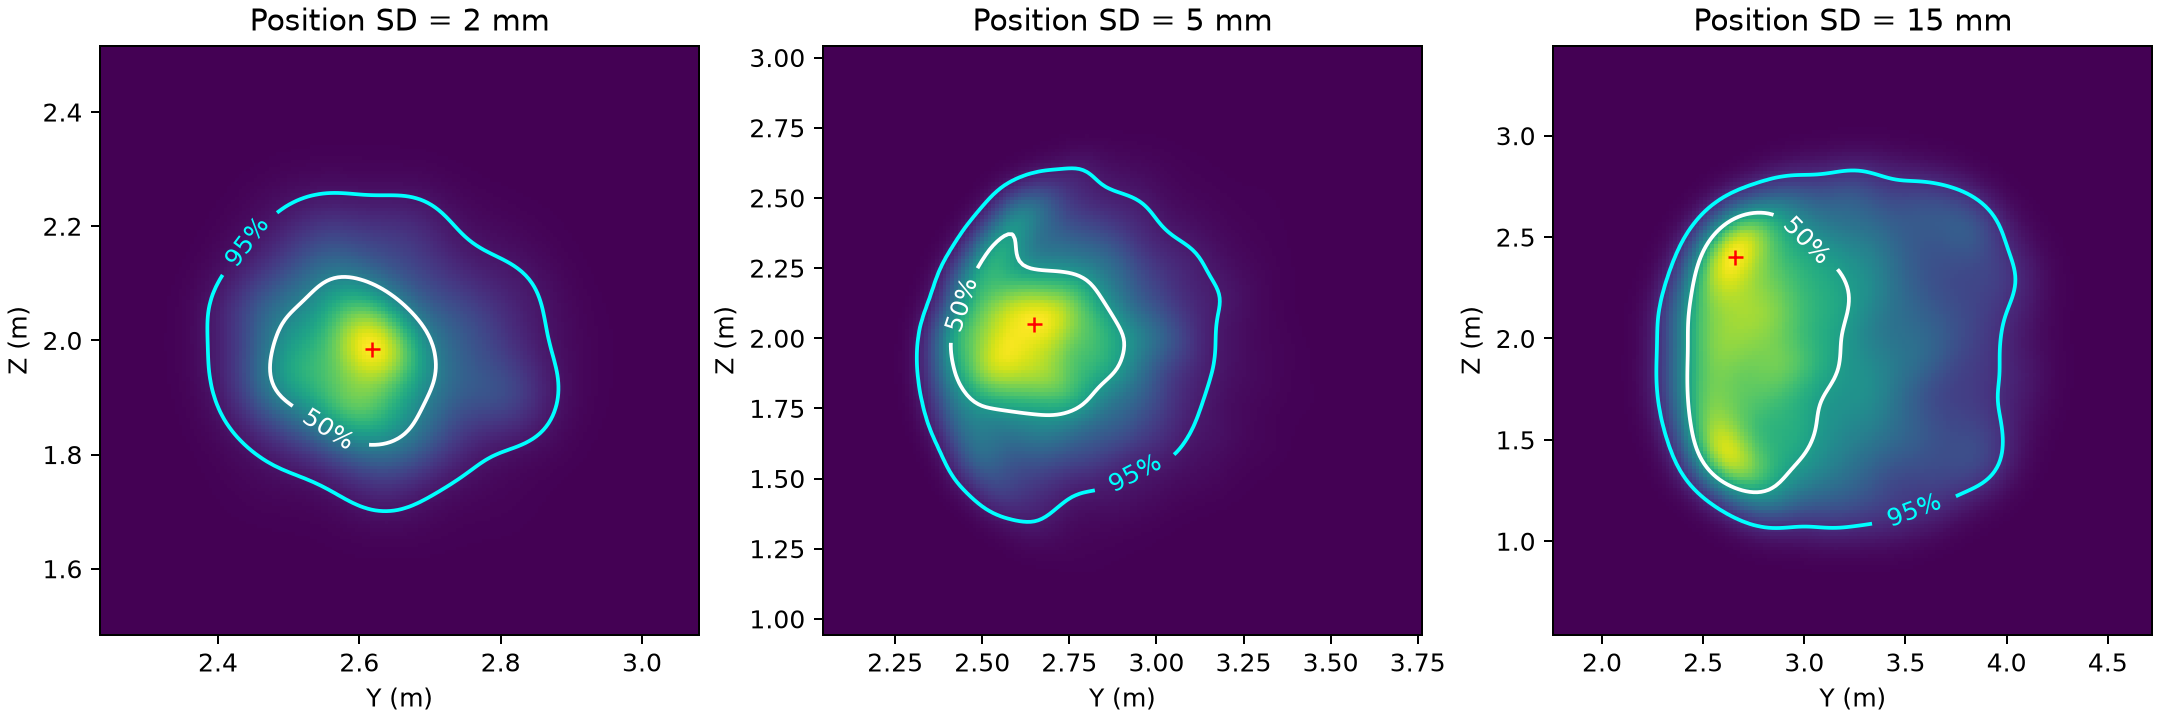
\includegraphics[width=\linewidth]{figures/case_regions.png}
  \caption{Joint posterior density of the goal-plane crossing $(Y,Z)$ for the stated case at $\sigma=2$, $5$ and $15\,\mathrm{mm}$ (left to right). White and cyan contours are the $50\%$ and $95\%$ highest-density regions from weighted kernel density estimation; crosses mark the grid mode. The grid includes off-target outcomes; no mass is truncated at the goal rectangle.}
  \label{fig:case}
\end{figure}

\begin{table}[htbp]
  \centering
  \caption{Posterior summary for the stated case at three observation noise levels (40{,}000 importance samples per stage, seed 8047). Areas are joint HDR areas; ESS is the effective sample size of the final weighted sample.}
  \label{tab:case}
  \begin{tabular}{rrrrrr}
    \toprule
    $\sigma$ (mm) & Mode $Y$ (m) & Mode $Z$ (m) & $50\%$ area ($\mathrm{m^2}$) & $95\%$ area ($\mathrm{m^2}$) & ESS \\
    \midrule
    2  & 2.617 & 1.984 & 0.051 & 0.207 & 124 \\
    5  & 2.650 & 2.052 & 0.219 & 0.809 & 2{,}893 \\
    15 & 2.657 & 2.400 & 0.841 & 2.645 & 5{,}744 \\
    \bottomrule
  \end{tabular}
\end{table}

The MDN, evaluated on the same noisy inputs, gives a mean crossing of $(2.773,1.924)\,\mathrm{m}$, a grid mode of $(2.759,1.899)\,\mathrm{m}$ and a goal probability of $0.974$. The two estimators therefore agree on the goal probability to about one percentage point, and their most likely points differ by about $0.1\,\mathrm{m}$ in each coordinate. This difference is a useful measure of model-form uncertainty: the MDN is sharper because it is trained on the simulation distribution, whereas the Bayesian posterior carries the full width of the drag and spin prior.

\subsection{Accuracy and Calibration on Held-Out Simulations}

Table~\ref{tab:holdout} reports the paired comparison on $4{,}187$ held-out trajectories. The constant-acceleration baseline degrades quickly with noise: its median error grows from $0.190\,\mathrm{m}$ at $2\,\mathrm{mm}$ to $1.217\,\mathrm{m}$ at $15\,\mathrm{mm}$, and it fails to produce a finite crossing in $6$ and $217$ cases at $5$ and $15\,\mathrm{mm}$ respectively. The current MDN reduces the median error to $0.163$, $0.322$ and $0.556\,\mathrm{m}$ at the three noise levels, $14\%$, $25\%$ and $54\%$ below the baseline. The previous network, trained on the same data volume with the earlier aerodynamic parameters, is consistently worse on the paired subset ($0.232$, $0.403$ and $0.656\,\mathrm{m}$), which confirms that the parameter update and the corrected lift direction improved the fit.

\begin{table}[htbp]
  \centering
  \small
  \caption{Held-out performance on $4{,}187$ airborne crossings (median Euclidean endpoint error in metres). The baseline fails to cross the plane for $0$, $6$ and $217$ cases at $\sigma=2$, $5$ and $15\,\mathrm{mm}$; all comparisons use the common valid subset. Coverage and area refer to the current MDN.}
  \label{tab:holdout}
  \begin{tabular}{rccccccc}
    \toprule
    $\sigma$ (mm) & Baseline & Previous MDN & Current MDN & $50\%$ cov. & $95\%$ cov. & $50\%$ area & $95\%$ area \\
    \midrule
    2  & 0.190 & 0.232 & \textbf{0.163} & 58.6\% & 97.6\% & 0.159 & 0.743 \\
    5  & 0.432 & 0.403 & \textbf{0.322} & 52.3\% & 96.3\% & 0.432 & 1.897 \\
    15 & 1.217 & 0.656 & \textbf{0.556} & 46.5\% & 96.8\% & 0.942 & 3.450 \\
    \bottomrule
  \end{tabular}
\end{table}

Calibration is mixed. The $95\%$ regions are close to nominal at all noise levels ($96.3$--$97.6\%$), but the $50\%$ regions are too wide at $2\,\mathrm{mm}$ ($58.6\%$ coverage) and slightly too narrow at $15\,\mathrm{mm}$ ($46.5\%$). The network therefore captures the overall scale of the uncertainty but not its shape at the median level; this is the main calibration defect of the present model and the reason we do not claim calibrated $50\%$ regions in the case study.

\subsection{Comparison with the Physics Posterior on Fresh Trajectories}

To test the estimators on trajectories that were not used to fit the MDN, twelve fresh trajectories were generated for each of two scenarios, and all three methods were evaluated on identical noisy inputs (Table~\ref{tab:benchmark}). With still air, the MDN and the physics posterior have comparable median errors ($0.341$ and $0.353\,\mathrm{m}$), both better than the baseline ($0.425\,\mathrm{m}$). With a $3\,\mathrm{m\,s^{-1}}$ crosswind, the physics posterior is the most accurate ($0.266\,\mathrm{m}$), while the MDN degrades to $0.352\,\mathrm{m}$, close to its nominal-air value. The MDN never saw wind during training, so this is the expected failure mode of a purely learned model; the physics model, which integrates the wind explicitly, is more robust. The physics posterior also has the better energy score in both scenarios ($0.211$ vs $0.258$, and $0.169$ vs $0.233$), at a cost of about $3$--$4\,\mathrm{s}$ per case against $1.4$--$1.6\,\mathrm{ms}$ for the MDN.

\begin{table}[htbp]
  \centering
  \caption{Fresh-trajectory comparison (twelve trajectories per scenario; only cases where all methods produced a finite crossing are paired). Errors are median endpoint errors in metres; the energy score is a proper scoring rule (lower is better). Per-case runtimes are given in the text; physics inference uses $6{,}000$ samples per stage.}
  \label{tab:benchmark}
  \begin{tabular}{lcccccc}
    \toprule
    Scenario & Paired & Baseline & MDN & Physics & Energy (MDN) & Energy (physics) \\
    \midrule
    Still air & 9/12 & 0.425 & 0.341 & 0.353 & 0.258 & \textbf{0.211} \\
    Crosswind & 10/12 & 0.804 & 0.352 & \textbf{0.266} & 0.233 & \textbf{0.169} \\
    \bottomrule
  \end{tabular}
\end{table}

\subsection{Sensitivity to the Drag Prior}

Because the drag coefficient is the least constrained aerodynamic input, the case was re-run with the upper prior limit raised from $0.30$ to $0.45$. Three independent seeds were used at each setting, with $40{,}000$ samples per stage (Table~\ref{tab:cdprior}). The $50\%$ area changes by $+1.1\%$ and the $95\%$ area by $-0.5\%$, both smaller than the spread between seeds, and the posterior mean moves by about $2\,\mathrm{cm}$. Within this model, the reported regions are therefore insensitive to the upper drag limit; this does not establish insensitivity to other aerodynamic assumptions.

\begin{table}[htbp]
  \centering
  \caption{Sensitivity of the case posterior to the upper limit of the drag prior ($\sigma=5\,\mathrm{mm}$, three seeds, $40{,}000$ samples per stage). Ranges are minima and maxima over seeds; means are averages over seeds.}
  \label{tab:cdprior}
  \begin{tabular}{lccc}
    \toprule
    $C_D$ prior & $50\%$ area ($\mathrm{m^2}$) & $95\%$ area ($\mathrm{m^2}$) & Mean $(Y,Z)$ (m) \\
    \midrule
    $U[0.15,0.30]$ & 0.213 (0.205--0.219) & 0.806 (0.789--0.821) & (2.696, 1.988) \\
    $U[0.15,0.45]$ & 0.215 (0.210--0.222) & 0.802 (0.792--0.809) & (2.689, 1.971) \\
    \bottomrule
  \end{tabular}
\end{table}

\begin{figure}[htbp]
  \centering
  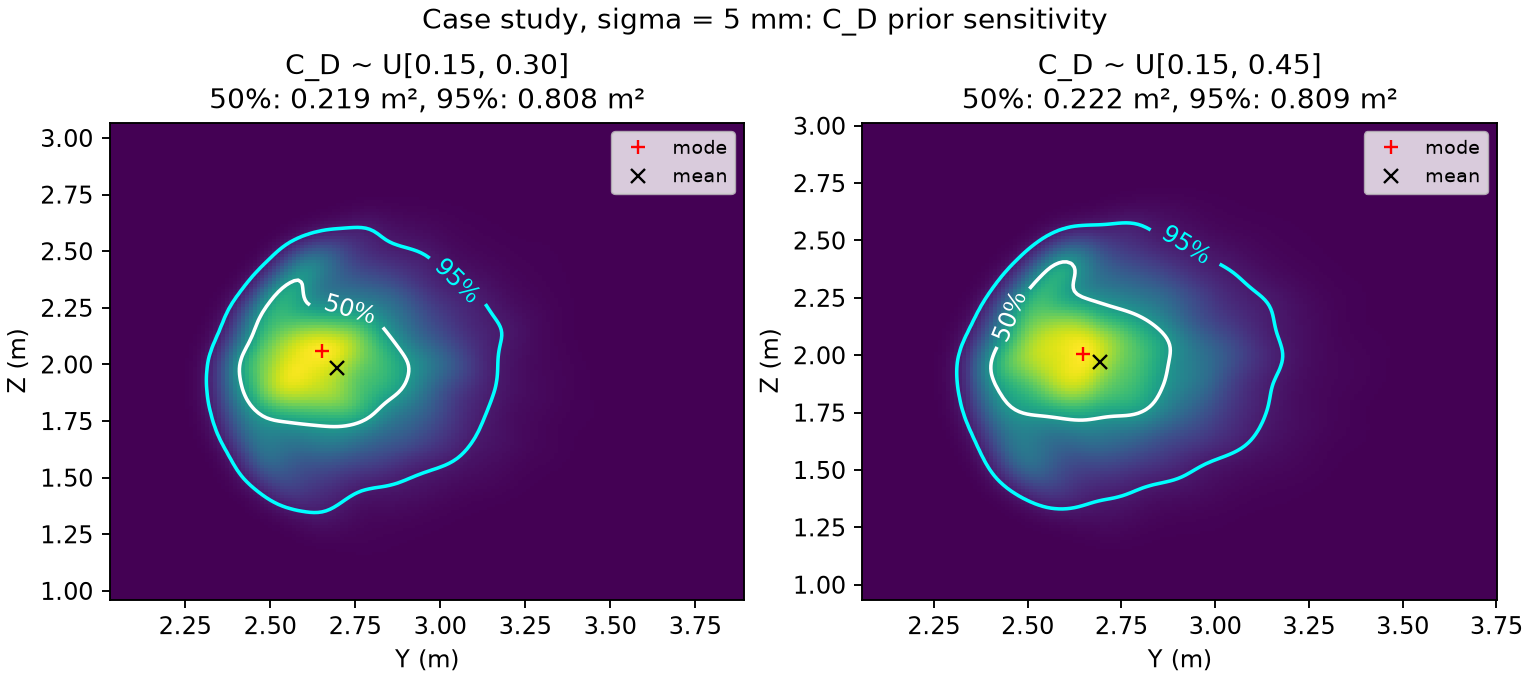
\includegraphics[width=\linewidth]{figures/cd_prior_contours.png}
  \caption{Case posterior at $\sigma=5\,\mathrm{mm}$ for the main drag prior (left) and the widened prior (right). Contours and areas are from one realisation (seed 8047); the three-seed means and ranges are given in Table~\ref{tab:cdprior}. The two regions are visually indistinguishable at the resolution of the plot.}
  \label{fig:cdprior}
\end{figure}

\subsection{Model-Form Check on Tracked Free-Kick Arcs}

The statistical evaluation above is entirely simulation-based. As an external check of the model form, we used two airborne arcs from the ISSIA-3D annotations \cite{soccernetv3d}, tracked at $25\,\mathrm{fps}$: frames 608--622 and 1144--1172, with the first six frames used to fit the initial state and the remaining frames held out. The arcs are free kicks and long passes, not penalties, and they carry centimetre-level reconstruction error; they can test the trajectory model but not the penalty prior.

Table~\ref{tab:issia} shows the held-out forecast RMSE. Gravity alone is clearly inadequate ($0.697$ and $2.179\,\mathrm{m}$). Adding quadratic drag with $C_D=0.22$ reduces the error to $0.489$ and $1.546\,\mathrm{m}$; $C_D=0.45$ gives $0.469$ and $1.584\,\mathrm{m}$, so the larger drag is not better on both arcs. A vertical net-lift term fitted on the prefix reduces the error further, to $0.188$ and $1.084\,\mathrm{m}$, with fitted $L=5.76\pm4.99$ and $6.89\pm3.83\,\mathrm{m\,s^{-2}}$ and fitted $C_D=0.363\pm0.169$ and $0.328\pm0.167$. This is evidence that a vertical force term is worth considering, but the fitted parameters are not identifiable at the precision needed for calibration, and the lift term may absorb tracking or reconstruction error. We therefore use these arcs only as a model-form check, not as a calibration set.

\begin{table}[htbp]
  \centering
  \caption{Held-out forecast error (RMSE, metres) for two ISSIA-3D airborne arcs. The first six frames of each arc are used to fit the initial state (and, for the last column, drag and vertical lift); later frames are held out. Final error is the error at the last observed frame.}
  \label{tab:issia}
  \begin{tabular}{llcccc}
    \toprule
    Arc & Quantity & Gravity & $C_D=0.22$ & $C_D=0.45$ & Drag + lift \\
    \midrule
    608--622 & Forecast RMSE & 0.697 & 0.489 & 0.469 & \textbf{0.188} \\
             & Final error   & 1.243 & 0.863 & 0.811 & \textbf{0.308} \\
    1144--1172 & Forecast RMSE & 2.179 & 1.546 & 1.584 & \textbf{1.084} \\
               & Final error   & 4.169 & 2.876 & 2.942 & \textbf{2.119} \\
    \bottomrule
  \end{tabular}
\end{table}

\section{Discussion}
\subsection{What the Two Estimators Agree On}

The Bayesian posterior and the MDN are built from different assumptions: one integrates the full nonlinear physics with an explicit prior, the other learns the mapping from examples. They nevertheless agree on the central prediction of the stated case to within about $0.1\,\mathrm{m}$ in $Y$, and on the goal probability to within about one percentage point ($0.963$ vs $0.974$). They also agree that constant acceleration is not the best point prediction: the baseline is $0.16\,\mathrm{m}$ from the posterior mode and $0.28\,\mathrm{m}$ from the MDN mean in $Y$. The agreement is reassuring, but it is agreement within one model family: both estimators share the same aerodynamic parameters, the same prior bounds and the same simulated training distribution.

The disagreement is also informative. The MDN is sharper than the posterior, with a higher goal probability and a smaller spread. This is expected from a network trained to minimise NLL on a fixed simulation distribution: it approximates the conditional distribution implied by that distribution, including any residual model error it has learned, while the Bayesian posterior propagates the full prior volume. Neither is automatically the better calibrated object; the held-out coverage in Table~\ref{tab:holdout} shows that the MDN's $50\%$ regions are not yet trustworthy, which is why the case study reports the Bayesian regions as the conservative choice.

\subsection{Strengths}

The method has four practical strengths. First, it returns a full predictive distribution, not a point estimate, so the answer includes the $50\%$ and $95\%$ regions and the goal probability that the problem asks for. Second, the physics model is transparent: every parameter has units, a literature source and a prior range, and the effect of changing the drag prior can be checked directly (Table~\ref{tab:cdprior}). Third, the MDN amortises the inference: once trained, it produces a distribution in about $1.5\,\mathrm{ms}$, which makes large-scale sensitivity studies and near-real-time use feasible. Fourth, the evaluation protocol is paired and clearly separated by trajectory, so the comparison between the baseline, the previous network and the current network is not confounded by different test data.

\subsection{Limitations and Applicability}

Several limitations must be stated plainly. The training data are simulated from the same prior that the Bayesian model uses; the reported coverages therefore measure self-consistency, not agreement with real penalties. The prior is a plausibility range, not a calibrated distribution of professional penalty kicks, and the goal probability inherits that choice. The MDN is conditioned on airborne arrival: a kicked ball that hits the ground before the goal line is outside its training target, and the reported probabilities are conditional on the ball reaching the plane in flight.

The benchmark in Table~\ref{tab:benchmark} is small (twelve trajectories per scenario, nine and ten paired), so the ranking between the MDN and the physics posterior in still air is within sampling noise. The MDN also has no wind input; its crosswind error is a genuine distribution-shift failure, not a tuning issue. The calibration of the $50\%$ regions is incomplete, and the $2\,\mathrm{mm}$ case has a low ESS ($124$), so its areas should be read as indicative. The event location uses linear interpolation at a $2\,\mathrm{ms}$ step; the step-refinement check bounds this error well below the observation noise, but it is not an exact root finder.

Finally, the external check uses two free-kick arcs, not penalties. Tracked penalty data from elite matches (the German Bundesliga dataset \cite{dfl2025} and the 2022 World Cup release \cite{pff2022}) are available for case-level testing, but they lack an independent launch time and a measured spin vector, and their ball-centre errors are not calibrated. They can support a case-by-case sanity check of the extrapolation, not the error statistics or coverages reported here. The present paper is therefore a calibrated simulation study with a model-form check on real flight, not a validated penalty predictor.

\section{Conclusion}

Two early positions and a known start are enough to produce a probabilistic answer to the penalty problem, provided the noise amplification is treated explicitly and the aerodynamic uncertainty is carried through the calculation. For the stated case, constant acceleration gives $T=0.405\,\mathrm{s}$ and $(Y,Z)=(2.495,1.920)\,\mathrm{m}$; the physics posterior gives a mode of $(2.650,2.052)\,\mathrm{m}$ with $50\%$ and $95\%$ joint regions of $0.219$ and $0.809\,\mathrm{m^2}$ and a goal probability of $0.963$. The noise-conditioned MDN gives $(2.773,1.924)\,\mathrm{m}$ and $0.974$ in about $1.5\,\mathrm{ms}$. On $4{,}187$ held-out trajectories the MDN reduces the median endpoint error by $14$--$54\%$ relative to constant acceleration and holds $95\%$ coverage at $96$--$98\%$, while the $50\%$ regions remain miscalibrated. Two tracked free-kick arcs support the drag correction and show that a vertical force term improves the forecast, but they cannot calibrate the penalty model. The immediate next step is to repeat the evaluation with calibrated, penalty-specific tracking data; until then, the numbers reported here should be read as simulation-calibrated predictions with honest uncertainty.

% References are numbered in the order you put them here. Every item should
% correspond to an actual source and be cited in the text with \cite{key}.
\begin{thebibliography}{99}
\bibitem{ifab} International Football Association Board, \emph{Laws of the Game 2025/26}, Laws 1 and 2 (field dimensions, penalty mark, ball). \url{https://www.theifab.com/laws/latest/}.
\bibitem{asai2007} T. Asai, K. Seo, O. Kobayashi, and R. Sakashita, ``Fundamental aerodynamics of the soccer ball,'' \emph{Sports Engineering} \textbf{10}(2), 101--109 (2007). \url{https://doi.org/10.1007/BF02844207}.
\bibitem{asai2013} T. Asai and K. Seo, ``Aerodynamic drag of modern soccer balls,'' \emph{SpringerPlus} \textbf{2}, 171 (2013). \url{https://doi.org/10.1186/2193-1801-2-171}.
\bibitem{goff2010} J. E. Goff and M. J. Carr\'e, ``Soccer ball lift coefficients via trajectory analysis,'' \emph{European Journal of Physics} \textbf{31}(4), 775--784 (2010). \url{https://doi.org/10.1088/0143-0807/31/4/007}.
\bibitem{goff2017} J. E. Goff, J. Kelley, C. M. Hobson, K. Seo, T. Asai, and S. B. Choppin, ``Creating drag and lift curves from soccer trajectories,'' \emph{European Journal of Physics} \textbf{38}(4), 044003 (2017). \url{https://doi.org/10.1088/1361-6404/aa6fcd}.
\bibitem{bray2003} K. Bray and D. Kerwin, ``Modelling the flight of a soccer ball in a direct free kick,'' \emph{Journal of Sports Sciences} \textbf{21}(2), 75--85 (2003). \url{https://doi.org/10.1080/0264041031000070994}.
\bibitem{kingma2015} D. P. Kingma and J. Ba, ``Adam: A method for stochastic optimization,'' in \emph{Proceedings of the 3rd International Conference on Learning Representations} (ICLR, 2015); arXiv:1412.6980.
\bibitem{soccernetv3d} M. Guti\'errez-P\'erez and A. Agudo, ``SoccerNet-v3D: Leveraging sports broadcast replays for 3D scene understanding,'' arXiv:2504.10106 (2025). \url{https://arxiv.org/abs/2504.10106}.
\bibitem{dfl2025} M. Bassek, R. Rein, H. Weber, and D. Memmert, ``An integrated dataset of spatiotemporal and event data in elite soccer,'' \emph{Scientific Data} \textbf{12} (2025). \url{https://doi.org/10.1038/s41597-025-04505-y}.
\bibitem{pff2022} PFF FC, ``Enhanced 2022 World Cup dataset'' (2023). \url{https://www.blog.fc.pff.com/blog/enhanced-2022-world-cup-dataset}.
\bibitem{bishop1994} C. M. Bishop, ``Mixture density networks,'' Technical Report NCRG/94/004, Aston University (1994).
\bibitem{gum2008} Joint Committee for Guides in Metrology, \emph{Evaluation of Measurement Data---Guide to the Expression of Uncertainty in Measurement}, JCGM 100:2008.
\bibitem{hyndman1996} R. J. Hyndman, ``Computing and graphing highest density regions,'' \emph{The American Statistician} \textbf{50}(2), 120--126 (1996). \url{https://doi.org/10.1080/00031305.1996.10474359}.
\bibitem{gneiting2007} T. Gneiting and A. E. Raftery, ``Strictly proper scoring rules, prediction, and estimation,'' \emph{Journal of the American Statistical Association} \textbf{102}(477), 359--378 (2007). \url{https://doi.org/10.1198/016214506000001437}.
\bibitem{harris2020} C. R. Harris et al., ``Array programming with NumPy,'' \emph{Nature} \textbf{585}, 357--362 (2020). \url{https://doi.org/10.1038/s41586-020-2649-2}.
\bibitem{virtanen2020} P. Virtanen et al., ``SciPy 1.0: fundamental algorithms for scientific computing in Python,'' \emph{Nature Methods} \textbf{17}, 261--272 (2020). \url{https://doi.org/10.1038/s41592-019-0686-2}.
\bibitem{paszke2019} A. Paszke et al., ``PyTorch: An imperative style, high-performance deep learning library,'' in \emph{Advances in Neural Information Processing Systems} \textbf{32}, 8024--8035 (2019).
\bibitem{hunter2007} J. D. Hunter, ``Matplotlib: A 2D graphics environment,'' \emph{Computing in Science \& Engineering} \textbf{9}(3), 90--95 (2007). \url{https://doi.org/10.1109/MCSE.2007.55}.
\end{thebibliography}
\addcontentsline{toc}{section}{References}

\appendix
\section{Propagation of Position Noise to Acceleration}
\label{app:noise}

Let the start $\mathbf{r}_0$ be exact and let the two observations be
\begin{equation}
  \mathbf{r}_1=\mathbf{r}_0+\mathbf{v}\Delta t+\tfrac12\mathbf{a}\Delta t^2+\boldsymbol{\varepsilon}_1,
  \qquad
  \mathbf{r}_2=\mathbf{r}_0+2\mathbf{v}\Delta t+2\mathbf{a}\Delta t^2+\boldsymbol{\varepsilon}_2,
\end{equation}
with independent errors of variance $\sigma^2$ per component. Eliminating $\mathbf{v}$ gives the second difference
\begin{equation}
  \mathbf{r}_2-2\mathbf{r}_1+\mathbf{r}_0
  =\mathbf{a}\Delta t^2+\boldsymbol{\varepsilon}_2-2\boldsymbol{\varepsilon}_1,
\end{equation}
whose component variance is $(1+4)\sigma^2=5\sigma^2$. Hence
\begin{equation}
  \sigma_a=\frac{\sqrt{5}\,\sigma}{\Delta t^2}.
\end{equation}
If the start is also noisy, the third error enters with unit weight and the variance becomes $6\sigma^2$, giving the conservative factor $\sqrt{6}$. At $\sigma=5\,\mathrm{mm}$ and $\Delta t=0.05\,\mathrm{s}$, $\sigma_a=4.47\,\mathrm{m\,s^{-2}}$ for a fixed start. Projected to the goal plane at $T\approx0.4\,\mathrm{s}$, the acceleration error alone displaces the crossing by roughly $\tfrac12\sigma_aT^2\approx0.37\,\mathrm{m}$, which is the same order as the differences between the models in this paper. This is why a point estimate without an uncertainty statement would be misleading, and why the prior bounds and the noise level must be carried through the inference.

% If required, the AI report must be the LAST section of the paper.
% Uncomment the following line after completing ai-report.tex.
% % If the official AI disclosure requirement applies, complete this file and
% uncomment % If the official AI disclosure requirement applies, complete this file and
% uncomment % If the official AI disclosure requirement applies, complete this file and
% uncomment \input{ai-report.tex} at the end of main.tex.
% Paste each exact query and complete output. Repeat for all relevant uses.
% Verbatim preserves line breaks and most special characters; a literal line
% containing \end{Verbatim} ends the block and must be handled separately.
\section*{Report on the Use of AI}
\addcontentsline{toc}{section}{Report on the Use of AI}

\noindent\textbf{System and how it was used:} [TODO: system name and use]

\noindent\textbf{Exact query:}
\begin{Verbatim}[breaklines=true,fontsize=\small]
[TODO: paste the complete, exact query]
\end{Verbatim}

\noindent\textbf{Full output:}
\begin{Verbatim}[breaklines=true,fontsize=\small]
[TODO: paste the complete output, without truncation]
\end{Verbatim}
 at the end of main.tex.
% Paste each exact query and complete output. Repeat for all relevant uses.
% Verbatim preserves line breaks and most special characters; a literal line
% containing \end{Verbatim} ends the block and must be handled separately.
\section*{Report on the Use of AI}
\addcontentsline{toc}{section}{Report on the Use of AI}

\noindent\textbf{System and how it was used:} [TODO: system name and use]

\noindent\textbf{Exact query:}
\begin{Verbatim}[breaklines=true,fontsize=\small]
[TODO: paste the complete, exact query]
\end{Verbatim}

\noindent\textbf{Full output:}
\begin{Verbatim}[breaklines=true,fontsize=\small]
[TODO: paste the complete output, without truncation]
\end{Verbatim}
 at the end of main.tex.
% Paste each exact query and complete output. Repeat for all relevant uses.
% Verbatim preserves line breaks and most special characters; a literal line
% containing \end{Verbatim} ends the block and must be handled separately.
\section*{Report on the Use of AI}
\addcontentsline{toc}{section}{Report on the Use of AI}

\noindent\textbf{System and how it was used:} [TODO: system name and use]

\noindent\textbf{Exact query:}
\begin{Verbatim}[breaklines=true,fontsize=\small]
[TODO: paste the complete, exact query]
\end{Verbatim}

\noindent\textbf{Full output:}
\begin{Verbatim}[breaklines=true,fontsize=\small]
[TODO: paste the complete output, without truncation]
\end{Verbatim}


\end{document}
